Based on the fact that most resource-demanding programs on edge cloud in our Sedgwick Natural Reserve settings are machine learning applications, in this section, we empirically evaluate Sparta's performance in a series of experiments on six benchmarks, ranging from image recognition, natural language processing to random forest and time series prediction, which are implemented based on Tensorflow and executed through Sparta's actuator interface. We first overview the machine learning benchmarks that we consider and our experimental methodology. We then present our results.

\subsection{Machine Learning Benchmarks}

To comprehensively evaluate the efficacy and efficiency of Sparta, we implemented 6 machine learning benchmarks, which consist of four categories: image recognition, natural language processing, ensemble learning and time series analysis. We aim to test Sparta on a variety of machine learning applications that represent different execution patterns.

\subsubsection{WTB\_Train}

is an image recognition application that we use as a benchmark to train a convolutional neural network (CNN)~\cite{ref:cnn} based on ResNet50~\cite{ref:resnet}. The training dataset contains animal images from a wildlife monitoring system called "Where's The Bear" (WTB)~\cite{ref:wtb}. "Where's The Bear" is an end-to-end distributed data acquisition and analytical system that automatically analyzes camera trap images collected by cameras sited at the Sedgwick Natural Reserve~\cite{ref:sedgwick} in Santa Barbara County, California. In total, there are five classes that we consider: Bear, Coyote, Deer, Bird, and Empty, by which we label images for training tasks. We also up-sampled minority classes using the Keras Image Data Generator~\cite{ref:datagen}, since the class size is unbalanced due to the frequency of animal occurrences. Doing so ensures that the classification model is not biased. We resized every image in the dataset to $1920 \times 1080$, and for each class, the dataset contains 60 images used to train the CNN model. Once the training is complete, the application stores this model in hdf5 format in object storage. 

The WTB\_Train application has a cold start at the beginning of the execution since it loads a pre-trained neural network model and training datasets. Once it completes loading, the entire training process has relatively consistent CPU usage and temperature. 

\subsubsection{WTB\_Inf}

inferences the type of wildlife in camera trap pictures based on the model trained by WTB\_Train. It loads the trained hdf5 model at the beginning and, for each picture, it assigns probabilities to five classes we consider in the training dataset by Softmax function. In each experiment, we assign 20 pictures for WTB\_Inf to inference. In terms of the execution pattern, WTB\_Inf runs in short bursts as opposed to WTB\_Train. Therefore, the CPU usage and temperature fluctuate dramatically throughout the execution of this benchmark.

\subsubsection{MNIST}

 is a dataset containing grayscale pictures of handwritten digits, in which it has 60,000 examples as the training set and 10,000 examples as the testing set. Based on the dataset, we train a 2-layer convolutional neural network~\cite{ref:MNIST} and test its accuracy in the third application. In contrast to WTB benchmarks, the size of pictures is smaller ($28 \times 28$) and the model is simplified in MNIST. 

\subsubsection{BiLSTM} is a sentiment analysis application based on a dataset of the Internet Movie Database (IMDB) movie reviews. It consists of 25,000 sequences each for training and testing. The model is constructed as a bidirectional LSTM with a classification layer using the sigmoid activation function. We train the model by the the training dataset and validate its performance in classifying sentiment by the testing dataset. Since it has a large dataset and a complex model, the execution pattern is long-running and consistent in CPU usage and temperature.


\subsubsection{Decision\_Forest} is an implementation of deep neural decision forests~\cite{ref:decision_forest} that classifies high-earning individuals from the pool. The benchmark leverages the United States Census Income Dataset~\cite{ref:uci} that has 48,843 instances with 14 features, including age, education, occupation, etc. The dataset is split up that the training part has 32,561 instances and the testing part has 16,282 instances. The application has three phases: it firstly processes the dataset by encoding input features. Then, it trains a deep neural decision tree model. Based on that, the application trains a neural decision forest model consists of a set of neural decision trees. Therefore, the usage and temperature of CPU increasingly grow throughout the process.


\subsubsection{Time\_Series} is a time series prediction application built on the climate data recorded by the Max Planck Institute for Biogeochemistry~\cite{ref:jena}. The dataset has 14 features such as temperature, pressure, humidity, etc. and the sampling frequency is 10 minutes. The time frame of the dataset ranges from Jan. 10th, 2009 to Dec. 31st, 2016. The application uses 300,693 rows to train a single-layer LSTM model, by which we can predict outdoor temperature in next 72 timestamps (12 hours) given the samples in the past 720 timestamps (120 hours). By this benchmark, we intend to evaluate Sparta on an application with a lightweight model and a large dataset.

% Execution pattern table

\subsection{Experimental Setup}

Each edge cloud node used in the experiments is an Intel NUC~\cite{ref:nuc} (6i7KYK) with two Intel Core i7-6770HQ 4-core processors (6M Cache, 2.60 GHz) and 32GB of DDR4-2133+ RAM connected via two channels. We use dynamic voltage and frequency scaling (DVFS) to control the frequency of CPU from 0.8GHz to 3.5GHz.

To simulate the natural temperature in Sedgwick natural reserve, we create three thermal environments in an isolated cooler that represent cold, neutral, and hot ambient temperature. In the cold scenario, the ambient temperature is 2.6\degree C and the CPU of NUC runs under 40\degree C in idle status. In the neutral scenario, the CPU of NUC starts at 51\degree C under the ambient temperature of 23.9\degree C. The hot scenario increases the ambient and CPU temperature to 43.8\degree C and 68\degree C respectively.

\begin{figure}
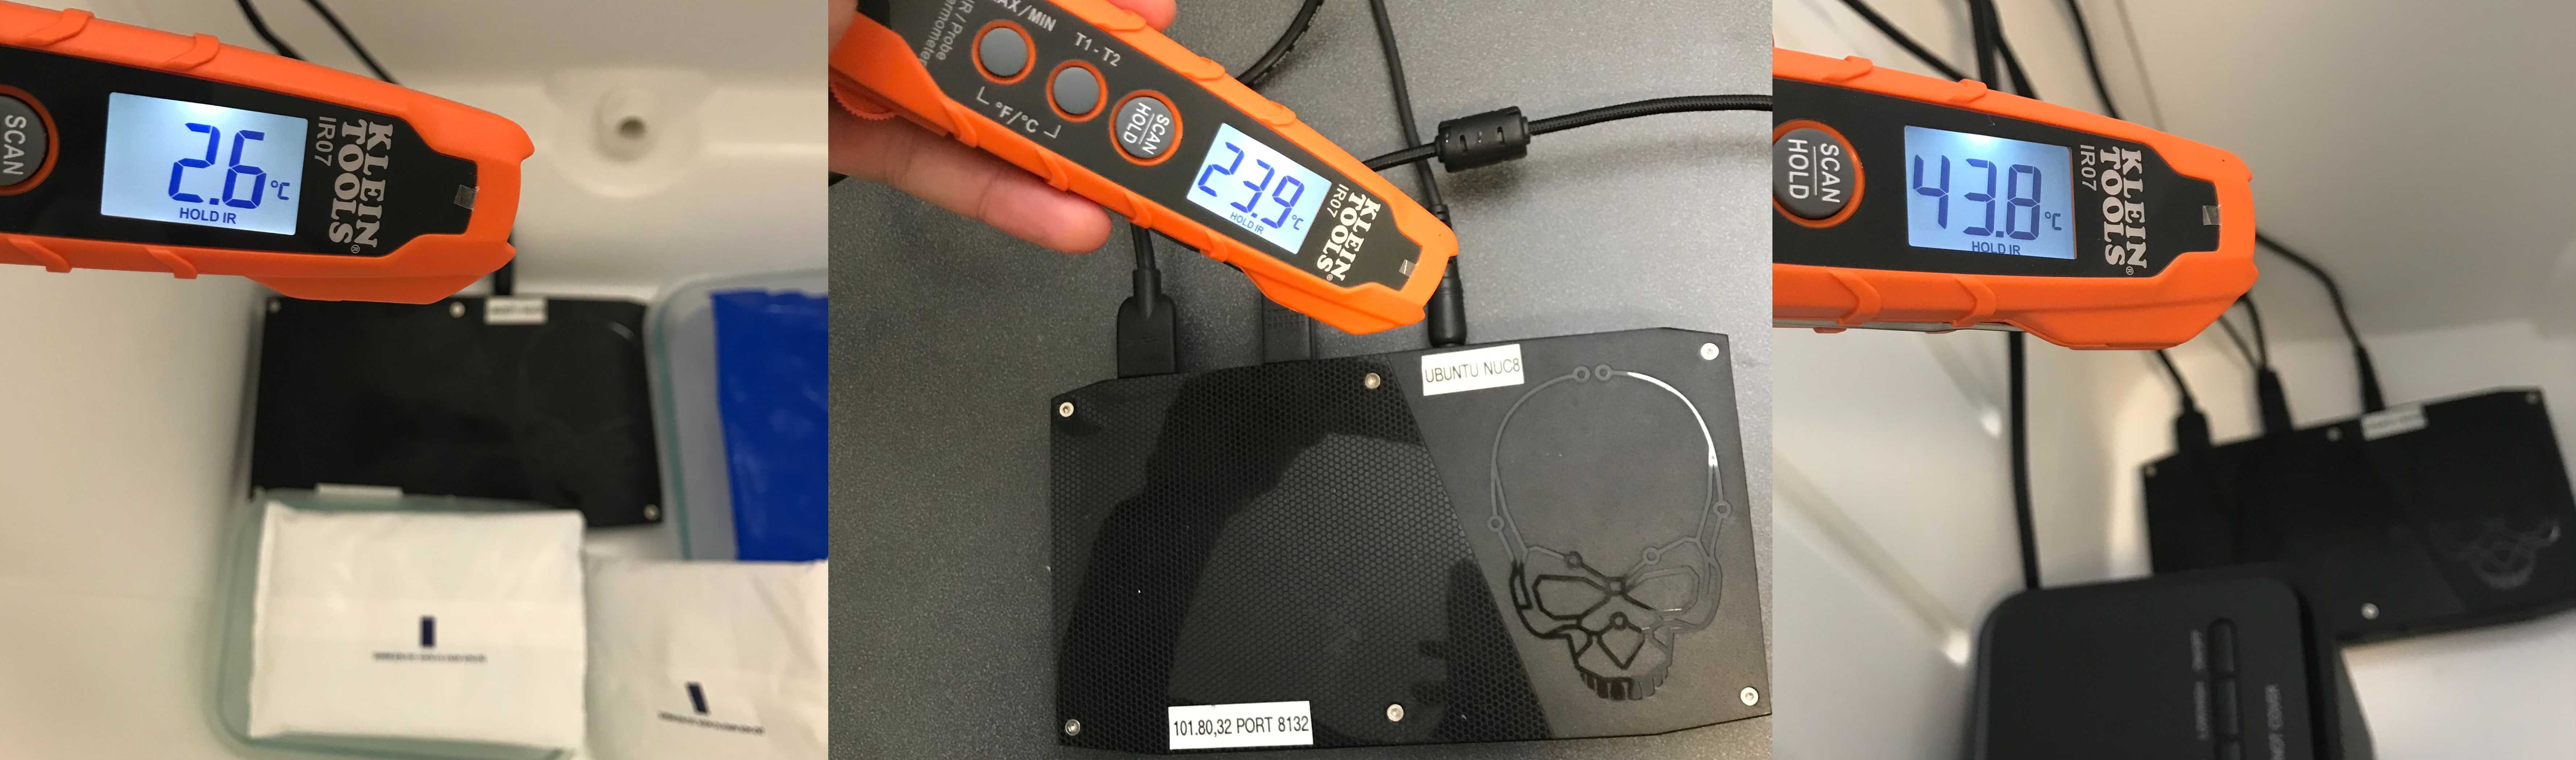
\includegraphics[width=\textwidth]{figures/thermal.jpg}
\caption{Three thermal environments in the experiment} \label{cold}
\end{figure}

There are two goals of the Sparta scheduler: the first is to limit the CPU temperature under the threshold; the second is to accelerate tasks without overheating the edge cloud. To evaluate these two objectives, we execute 6 machine learning benchmarks under 3 modes of Sparta scheduler. In each experiment, Sparta takes inputs of task program, corresponding workload dataset and a threshold temperature. To keep the comparison consistent across 3 thermal environments, we use 75\degree C as the threshold temperature for all experiments.

In 3 modes of Sparta, we execute each machine learning benchmark repeatedly 100 times under 3 thermal environments (totally $3 \times 3 \times 6 \times 100 = 5400$ executions) and report relevant metrics, both mean and standard deviation, to compare the efficacy and efficiency among Annealing, AIMD, and Hybrid modes.


\subsection{Application Efficacy}

We first measure the stabilization time for six benchmarks. We define stabilization time as the elapsed time from the start to the point all CPU temperatures in the sampling time window are within $[T_s - T_d, T_s]$, where $T_s$ is the threshold and $T_d$ is a slack variable (3 \degree C by default). During each of the 10 consecutive executions (1 epoch) of benchmarks, we record the duration when the Sparta scheduler stabilizes the CPU temperature according to the threshold. As shown in the first part of Table \ref{tab:stab}, we report the mean and stdev of stabilization time for each benchmark in 3 modes. Hybrid mode uses less time to stabilize CPU temperature than Annealing and AIMD in all six benchmarks. It performs even better in WTB\_Inf benchmark that has a short burst execution pattern and volatile CPU temperature.

%Stabilization table

\begin{table}[t]
\caption{The mean and stdev of \textbf{stabilization time} in seconds for 6 machine learning benchmarks in 3 Sparta modes. Compared to Annealing and AIMD, Hybrid mode uses less time to stabilize CPU temperature across all benchmarks and all thermal scenarios. }\label{tab:stab}
\vspace{1mm}
\centering
\resizebox{350pt}{!}{\begin{tabular}{
|>{\centering}m{2cm}
|>{\centering}m{2cm}
|>{\centering}m{2cm}
|>{\centering}m{2cm}
|>{\centering}m{2cm}
|>{\centering}m{2cm}
|>{\centering\arraybackslash}m{2cm}|}
\hline
\rowcolor{Gray}
& {\bfseries WTB Train} & {\bfseries WTB Inf} & {\bfseries MNIST} & {\bfseries BiLSTM} & {\bfseries Decision Forest} & {\bfseries Time Series}\\
\hline
{\bfseries Annealing} & 53.79 (30.1) & 50.7 (21.1) & 62.02 (32.2) & 69.02 (33.8) & 59.13 (31.9) & 72.31 (28.8) \\

{\bfseries AIMD} & 61.73 (24.9) & 63.26 (25.0) & 58.91 (14.0) & 59.9 (11.2) & 78.17 (30.7) & 73.41 (28.9) \\

{\bfseries Hybrid} & \color{red}38.59 (26.11) & \color{red}23.24 (17.33) & \color{red}38.66 (22.17) & \color{red}52.83 (20.6) & \color{red}55.46 (25.5) & \color{red}52.91 (29.8) \\
\hline

\end{tabular}
}
\newline
\vspace{3mm}
\newline
\resizebox{300pt}{!}{\begin{tabular}{
|>{\centering}m{2cm}
|>{\centering}m{2cm}
|>{\centering}m{2cm}
|>{\centering}m{2cm}
|>{\centering\arraybackslash}m{2cm}|}
\hline
\rowcolor{Gray}
& {\bfseries Neutral} & {\bfseries Cold} & {\bfseries Hot} & {\bfseries Average} \\
\hline
{\bfseries Annealing} & 68.15 & 67.27 & 48.07 & 61.16 \\

{\bfseries AIMD} & 63.10 & 77.40 & 57.20 & 65.90  \\

{\bfseries Hybrid} & \color{red}43.03 & \color{red}52.43 & \color{red}35.39 & \color{red}43.61 \\
\hline
\end{tabular}
}
\end{table}


%Runtime table


As the second part of Table \ref{tab:stab} presents the result in the thermal dimension, Hybrid mode also uses less time to stabilize CPU temperature across all 3 thermal environments, comparing to Annealing and AIMD. Averagely, Hybrid mode uses 43.61 seconds in the stabilization phase, in contrast to 61.16 seconds in Annealing and 65.9 seconds in AIMD. Hybrid mode's performance is even better in the hot scenario, which is the key use case for edge devices to prevent overheating in Sedgwick natural reserve.

\begin{table}[t]
\caption{The mean and stdev of \textbf{execution time} in seconds for 6 machine learning benchmarks in 3 modes of Sparta. Compared to Annealing and AIMD, Hybrid mode uses less time to complete tasks across all benchmarks and all thermal scenarios. }\label{tab:runtime}
\vspace{1mm}
\centering
\resizebox{350pt}{!}{\begin{tabular}{
|>{\centering}m{2cm}
|>{\centering}m{2cm}
|>{\centering}m{2cm}
|>{\centering}m{2cm}
|>{\centering}m{2cm}
|>{\centering}m{2cm}
|>{\centering\arraybackslash}m{2cm}|}
\hline
\rowcolor{Gray}
& {\bfseries WTB Train} & {\bfseries WTB Inf} & {\bfseries MNIST} & {\bfseries BiLSTM} & {\bfseries Decision Forest} & {\bfseries Time Series}\\
\hline
{\bfseries Annealing} & 374.67 (9.8) & 60.94 (3.9) & 39.85 (2.9) & 222.34 (3.5) & 48.21 (3.6) & 130.65 (7.6) \\

{\bfseries AIMD} & 393.55 (5.8) & 64.32 (3.9) & 36.51 (4.3) & 234.92 (5.2) & 45.38 (2.2) & 110.06 (6.2) \\

{\bfseries Hybrid} & \color{red}318.55 (4.2) & \color{red}55.31 (3.2) & \color{red}32.53 (2.3) & \color{red}212.91 (2.6) & \color{red}41.56 (4.4) & \color{red}98.78 (7.2) \\
\hline
\end{tabular}
}
\newline
\vspace{3mm}
\newline
\resizebox{300pt}{!}{\begin{tabular}{
|>{\centering}m{2cm}
|>{\centering}m{2cm}
|>{\centering}m{2cm}
|>{\centering}m{2cm}
|>{\centering\arraybackslash}m{2cm}|}
\hline
\rowcolor{Gray}
& {\bfseries Neutral} & {\bfseries Cold} & {\bfseries Hot} & {\bfseries Average} \\
\hline
{\bfseries Annealing} & 145.72 & 116.14 & 176.42 & 146.09 \\

{\bfseries Speedup} & 1.17x & 1.06x & 1.26x & \color{red}1.16x \\

\hline

{\bfseries AIMD} & 134.67 & 122.28 & 185.42 & 147.46  \\

{\bfseries Speedup} & 1.07x & 1.15x & 1.18x & \color{red}1.14x  \\

\hline

{\bfseries Hybrid} & \color{red}124.86 & \color{red}107.68 & \color{red}147.28 & \color{red}126.61 \\
\hline
\end{tabular}
}
\end{table}


We next empirically evaluate the execution time of six benchmarks by the Sparta scheduler. In the first part of Table \ref{tab:runtime}, we report the mean and stdev of execution time for each benchmark under 3 modes. On average, the Hybrid mode completes the task of each benchmark faster than Annealing and AIMD. Given the stdev and degree of freedom, we also run student t-test among 3 modes for each benchmark and confirm that the execution time by Hybrid is smaller than Annealing and AIMD with a statistical significance level of 5\%. Table \ref{tab:runtime} also indicates the speedup of Hybrid over Annealing and AIMD, ranging from 1.04x to 1.32x. 

The second part of Table \ref{tab:runtime} demonstrates the average execution time in 3 thermal scenarios. On average, Hybrid mode completes the task in 126.61 seconds, in comparison with 146.09 seconds by Annealing and 147.46 seconds by AIMD. Hybrid mode provides 1.16x and 1.14x speedup respectively over Annealing and AIMD. These results show that Sparta in Hybrid mode efficiently executes more workloads than Annealing and AIMD mode under the same temperature threshold. 


%RSME of all temp table

\begin{table}[t]
\caption{The mean and stdev of \textbf{RMSE} of all temperature samples for 6 benchmarks in 3 modes of Sparta. Compared to Annealing and AIMD, Hybrid mode has less RSME to threshold temperature across all benchmarks and all thermal scenarios.}\label{tab:rsme}
\vspace{1mm}
\centering
\resizebox{350pt}{!}{\begin{tabular}{
|>{\centering}m{2cm}
|>{\centering}m{2cm}
|>{\centering}m{2cm}
|>{\centering}m{2cm}
|>{\centering}m{2cm}
|>{\centering}m{2cm}
|>{\centering\arraybackslash}m{2cm}|}
\hline
\rowcolor{Gray}
& {\bfseries WTB Train} & {\bfseries WTB Inf} & {\bfseries MNIST} & {\bfseries BiLSTM} & {\bfseries Decision Forest} & {\bfseries Time Series}\\
\hline
{\bfseries Annealing} & 5.04 (1.0) & 7.88 (1.7) & 9.22 (0.8) & 5.07 (1.3) & 9.91 (1.5) & 9.63 (2.4) \\

{\bfseries AIMD} & 4.39 (0.6) & 6.24 (0.9) & 8.35 (1.0) & 5.81 (2.1) & 9.95 (1.6) & 8.67 (3.1) \\

{\bfseries Hybrid} & \color{red}4.32 (0.6) & \color{red}5.79 (1.2) & \color{red}6.11 (1.8) & \color{red}4.90 (1.2) & \color{red}9.48 (2.4) & \color{red}7.25 (3.0) \\
\hline
\end{tabular}
}
\newline
\vspace{3mm}
\newline
\resizebox{300pt}{!}{\begin{tabular}{
|>{\centering}m{2cm}
|>{\centering}m{2cm}
|>{\centering}m{2cm}
|>{\centering}m{2cm}
|>{\centering\arraybackslash}m{2cm}|}
\hline
\rowcolor{Gray}
& {\bfseries Neutral} & {\bfseries Cold} & {\bfseries Hot} & {\bfseries Average} \\
\hline
{\bfseries Annealing} & 7.12 & 9.59 & 6.67 & 7.79 \\

{\bfseries AIMD} & 5.69 & 9.39 & 5.79 & 6.96  \\

{\bfseries Hybrid} & \color{red}4.92 & \color{red}9.10 & \color{red}4.99 & \color{red}6.34 \\
\hline
\end{tabular}
}
\end{table}


To investigate the error from the sampling temperature and threshold, we next evaluate the Root Mean Square Error (RMSE) of all temperature samples in the executions. We define $RMSE = \sqrt{\frac{1}{n}\sum_{i=1}^{n}(T_i - \hat{T})^2}$, where $T_i$ is a sample of CPU temperature, $\hat{T}$ is the temperature threshold and n is the number of temperature samples. In Table \ref{tab:rsme}, we display the mean and stdev of RMSE of all CPU temperature samples. The RMSE of Hybrid mode is the least across all six benchmarks among the other two modes. Hybrid mode also has the lowest RMSE in all three thermal scenarios. On average, Hybrid has 6.34 as RMSE for all temperature samples from the threshold. 

%Percentage of temp below threshold table

\begin{table}[t]
\caption{The mean and stdev of \textbf{PTBT} (Percentage of Temperature Below Threshold) for 6 benchmarks in 3 modes of Sparta. Due to their inherent algorithm, Annealing has the lowest PTBT value and AIMD has the highest, whereas the Hybrid mode has the PTBT value in-between across all benchmarks and all thermal scenarios.}\label{tab:percent}
\vspace{1mm}
\centering
\resizebox{350pt}{!}{\begin{tabular}{
|>{\centering}m{2cm}
|>{\centering}m{2cm}
|>{\centering}m{2cm}
|>{\centering}m{2cm}
|>{\centering}m{2cm}
|>{\centering}m{2cm}
|>{\centering\arraybackslash}m{2cm}|}
\hline
\rowcolor{Gray}
& {\bfseries WTB Train} & {\bfseries WTB Inf} & {\bfseries MNIST} & {\bfseries BiLSTM} & {\bfseries Decision Forest} & {\bfseries Time Series}\\
\hline
{\bfseries Annealing} & 71.8\% (0.05) & 83.0\% (0.14) & 83.4\% (0.09) & 72.6\% (0.10) & 84.3\% (0.07) & 91.0\% (0.13) \\

{\bfseries AIMD} & 97.2\% (0.07) & 99.7\% (0.01) & 98.0\% (0.08) & 99.6\% (0.09) & 98.7\% (0.04) & 99.5\% (0.25) \\

{\bfseries Hybrid} & 93.0\% (0.11) & 95.2\% (0.14) & 92.7\% (0.07) & 97.2\% (0.23) & 91.1\% (0.10) & 96.9\% (0.17) \\
\hline
\end{tabular}
}
\newline
\vspace{3mm}
\newline
\resizebox{300pt}{!}{\begin{tabular}{
|>{\centering}m{2cm}
|>{\centering}m{2cm}
|>{\centering}m{2cm}
|>{\centering}m{2cm}
|>{\centering\arraybackslash}m{2cm}|}
\hline
\rowcolor{Gray}
& {\bfseries Neutral} & {\bfseries Cold} & {\bfseries Hot} & {\bfseries Average} \\
\hline
{\bfseries Annealing} & 88.3\% & 79.7\% & 75.1\% & 81.1\% \\

{\bfseries AIMD} & 99.7\% & 98.6\% & 98.2\% & 98.8\%  \\

{\bfseries Hybrid} & 98.1\% & 92.29\% & 92.7\% & 94.4\% \\
\hline
\end{tabular}
}
\end{table}


Lastly, we report the percentage of samples below threshold temperature in six benchmarks. The first part of Table \ref{tab:percent} manifests the mean and stdev of PTBT (Percentage of Temperature Below Threshold) for six benchmarks. Because Annealing mode uses a probabilistic algorithm, it results in the lowest PTBT metric among three modes. Since AIMD mode multiplicatively decreases the CPU frequency whenever a temperature over the threshold is detected, it has the highest PTBT metrics in all six benchmarks. Combined with Annealing and AIMD, the PTBT of Hybrid mode is between the other two modes. This relationship holds for all three thermal scenarios, as depicted in the second part of Table \ref{tab:percent}. Hybrid mode maintains 94.4\% of all temperature samples below the threshold. Thus, we consider the above results strong proofs of Sparta's efficacy in preventing overheating of edge devices and executing a variety of tasks as efficiently as possible.





